\chapter[Resultados Preliminares]{Resultados Preliminares}

\section{Primeiro Experimento}

A Tabela \ref{tab:tabela_guarda_de_inclusao} e a Figura 
\ref{grafico_guardas_de_inclusao} apresentam os resultados
 do primeiro experimento realizado, que avalia os impactos
 dos diferentes métodos de guarda de inclusão (Seção \ref{experimento_1}).


\begin{table}[!ht]
\centering
\caption{Repetições com Guardas de Inclusão}
\label{tab:tabela_guarda_de_inclusao}
\begin{tiny}
\begin{tabular}{lp{1.5cm}p{1.5cm}p{1.5cm}p{1.5cm}p{2cm}p{2cm}p{2cm}p{2cm}|}
\toprule
\textbf{Tipo} & \multicolumn{7}{l}{Utilização de Guarda de Inclusão} \\
\textbf{Medida} & \multicolumn{7}{l}{Tempos em segundos } \\
\textbf{Amostras} & \textbf{Guarda de Inclusão Externa} & \textbf{Guarda de Inclusão Interna} & \textbf{Pragma Once} & \textbf{Gua  rda de Inclusão Interna Primeiro que Pragma Once} & \textbf{Pragma Once primeiro que Guarda de Inclusão Interna} & \textbf{Guarda   de Inclusão Externa e Pragma Once} & \textbf{Redundância de Guarda de Inclusão} \\ \midrule
 1  & 7,22 & 7,09 & 13,95  &  14,20 &14,63   &  13,55 &  7,18  \\ \midrule
 2  & 7,26 & 6,98 & 13,77  &  14,38 & 14,36  &  13,46 & 7,10   \\ \midrule
 3  & 7,26 & 7,11 & 14,02  &  13,31 & 14,10  &  13,24 &7,09    \\ \midrule
 4  & 7,27 & 7,38 & 14,03  &  14,12 & 13,69  &  13,99 &6,25    \\ \midrule
 5  & 6,98 & 7,01 & 13,51  &  14,13 & 13,45  &  13,64 &6,81    \\ \midrule
 6  & 7,16 & 6,59 & 13,87  &  14,52 & 13,80  &  13,60 &6,57    \\ \midrule
 7  & 7,26 & 6,87 & 13,65  &  13,65 & 13,87  &  13,87 &6,85    \\ \midrule
 8  & 7,23 & 6,80 & 13,99  &  14,08 & 13,18  &  13,26 &6,85    \\ \midrule
 9  & 7,04 & 6,39 & 13,77  &  13,68 & 13,34  &  13,77 &6,99    \\ \midrule
 10 & 7,38 & 6,94 & 13,62  &  13,99 & 13,51  &  13,50 &6,81    \\ \midrule
 Média: & 7,21 & 6,92 & 13,82& 14,01& 13,79  &  13,59 &6,85    \\ \bottomrule
\end{tabular}
\end{tiny}
\end{table}
A Tabela \ref{tab:modelo_guards} representa o modelo utilizado na coleta dos dados.

Para os experimentos realizados com guardas de inclusão mostrados na 
Tabela \ref{tab:tabela_guarda_de_inclusao}, o menor tempo médio foi
 com a utilização do método redundante, fato  que corrobora a afirmação
 de John Lakos de que o método redundante é mais eficiente que a inclusão
 interna ou externa, em poucos segundos. Analisando a Figura 
\ref{grafico_guardas_de_inclusao} os maiores tempos de compilação foram 
 obtidos com a utilização do pragma once. Como dito anteriormente, este 
método está obsoleto em relação ao g++ e a diferença chega a quase 50\%
 em relação aos outros métodos.

\begin{figure}[h]
    \centering
        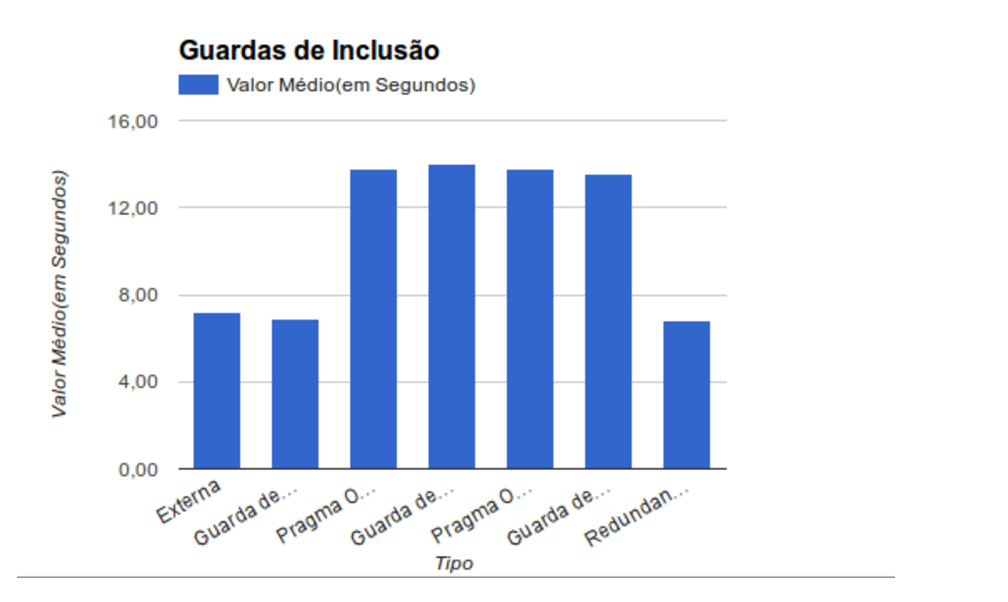
\includegraphics[keepaspectratio=true,scale=1]{figuras/guardas_de_inclusao.eps}
    \caption{Redução em segundos para cada método guarda de inclusão}
    \label{grafico_guardas_de_inclusao}
\end{figure}


\section{Segundo Experimento}


A Tabela \ref{experimento_02} e a Figura \ref{grafico_forward_declaration} apresentam os resultados do
 segundo experimento, que avalia o uso das \textit{forward declarations}.Fator de
 Redução é igual a 1 menos o tempo sem \textit{forward declaration} divido pelo
 tempo com \textit{forward declaration}.



\begin{table}[!ht]
\centering
\caption{Resultado das experimentos \textit{forward declaration}}
\label{experimento_02}
\begin{tabular}{lp{3cm}p{3cm}p{3cm}}
\toprule
\textbf{Tipo} & \multicolumn{3}{l}{Forward Declaration}\\ \midrule
\textbf{Tempo}& \multicolumn{3}{l}{Em segundos}    \\ \midrule
\textbf{Repetições} & \textbf{Sem forward Declaration(SFD)} & \textbf{Com Forward Declaration (CFD)} & \textbf{Fator de Redução (SFD/CFD)} \\ \midrule
1      & 5,11  & 5,042 & 1,3\% \\ \midrule
2      & 5,07  & 4,984 & 1,8\% \\ \midrule
3      & 5,12  & 5,055 & 1,3\% \\ \midrule
4      & 5,12  & 4,937 & 3,5\% \\ \midrule
5      & 5,18  & 5,153 & 0,5\% \\ \midrule
6      & 5,20  & 5,045 & 3,1\% \\ \midrule
7      & 5,15  & 4,986 & 3,1\% \\ \midrule
8      & 5,21  & 5,151 & 1,0\% \\ \midrule
9      & 5,21  & 5,045 & 3,1\% \\ \midrule
10     & 5,13  & 5,09  & 0,8\% \\ \midrule
Média  & 5,15  & 5,05  & 1,9\% \\ \bottomrule
\end{tabular}
\end{table}


\begin{figure}[h]
    \centering
        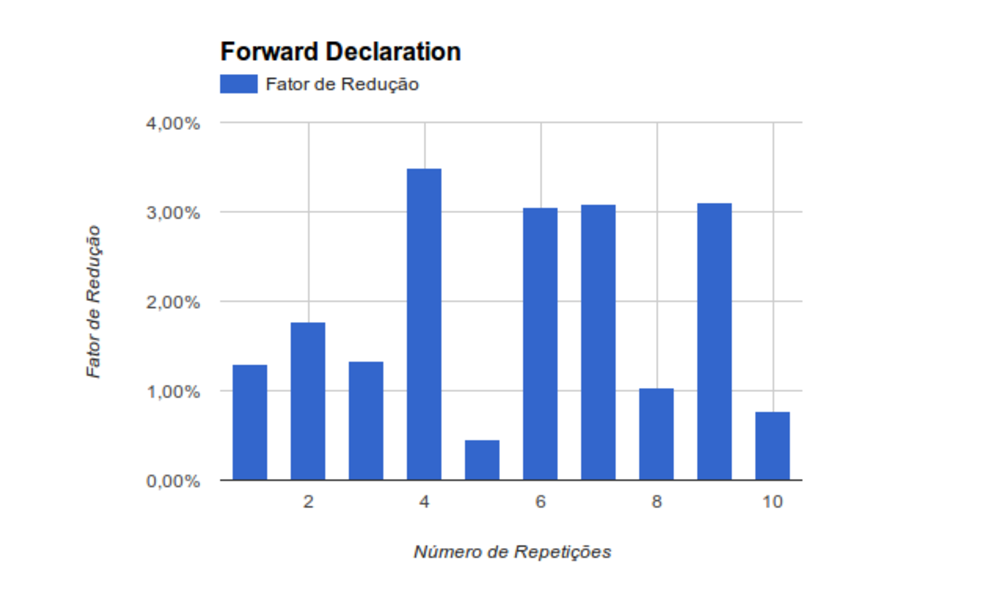
\includegraphics[keepaspectratio=true,scale=1]{figuras/forward_declaration.eps}
    \caption{Fator de redução para cada dado coletado \textit{forward declaration}}
    \label{grafico_forward_declaration}
\end{figure}
A Tabela \ref{experimento_02} mostra os valores coletados durante
 os experimentos de \textit{forward declaration}. O Gráfico
 \ref{grafico_forward_declaration} demonstra que todos os valores
 foram positivos, indicando que \textit{forward declaration} reduziu o tempo
 de compilação em todos os casos, com uma variação de 0,5\% a 3,1\%.

\begin{table}[!ht]
\centering
\caption{Resultado modificações parciais com \textit{foward declaration}, em segundos}
\label{amostas_experimento_03}
\begin{tabular}{p{3cm}p{3cm}p{3cm}p{3cm}}
\toprule
\textbf{Quantidade de Modificações} & \textbf{Sem forward Declaration}  & \textbf{Com forward Declaration} & \textbf{Fator de Redução}\\ \midrule
1  & 2,01 & 1,61 & 19,90\% \\ \midrule
15 & 4,2  & 3,48 & 17,14\% \\ \midrule
4  & 4,48 & 4,45 & 0,67\% \\  \midrule
1  & 2,01 & 1,56 & 22,39\% \\ \midrule
4  & 2,32 & 2,07 & 10,78\% \\ \midrule
12 & 4,44 & 4,46 & -0,45\% \\ \midrule
12 & 5,03 & 4,26 & 15,31\% \\ \midrule
8  & 4,83 & 4,38 & 9,32\% \\  \midrule
12 & 4,43 & 3,36 & 24,15\% \\ \midrule
4  & 4,38 & 4,31 & 1,60\% \\  \midrule
Média  & 3,81  & 3,39  & 10,99\% \\ \bottomrule 
\end{tabular}
\end{table}


\begin{figure}[h]
    \centering
        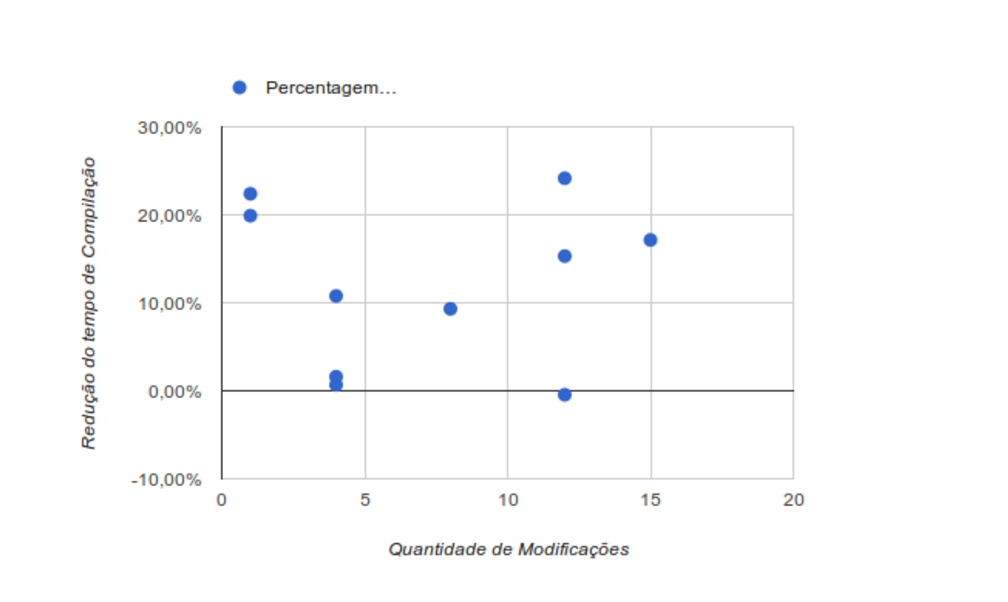
\includegraphics[keepaspectratio=true,scale=1]{figuras/forward_declaration2.eps}
    \caption{Dados utilizando script de modificações}
    \label{grafico_forward_declaration2}
\end{figure}
A Figura \ref{grafico_forward_declaration2} representa a utilização
 do Código \ref{script_forward_declaration},
 que realiza modificações na data de modificação de um arquivo, o que forca uma
 recompilação do mesmo na próxima invocação do comando make.
 Esta tabela mostra que realizando modificações em diferentes
 quantidades de arquivos o beneficio do \textit{forward declaration} é
 diretamente impactado. Ainda assim, apenas em uma amostra o percentual
 de redução foi negativo  (isto é, houve um acréscimo de tempo,
 em relação a média), no entanto com uma variação baixa.



\section{Terceiro Experimento}

O terceiro experimento avaliou o impacto da compilação
 paralela através do uso da flag \texttt{-j} do
 comando make (Seção \ref{experimento_03}).



\textbf{CPPCheck}:


\begin{table}[h]
\centering
\caption{CppCheck utilizando jobs do makefile}
\label{tab:cppcheck}
\begin{tiny}
\begin{tabular}{cccccccccc}
\toprule
\textbf{Repetições} & \multicolumn{9}{c}{\textbf{Número de threads}} \\ \midrule
- & 1 & 2 & 4 & 6 & 8 & 10 & 12 & 14 & 16 \\ 
1 & 156,55  &  117,06  &  99,49   &  89,60    & 100,10   & 110,24  & 95,44     & 104,99   & 136,11 \\ 
2 & 158,594 &  121,217 &  114,765 &  99,578   & 100,418  & 98,722  & 119,161   & 117,518  & 113,762 \\ 
3 & 148,788 &  122,364 &  117,067 &  112,585  & 98,579   & 95,049  & 114,737   & 102,282  & 101,268 \\ 
4 & 150,221 &  127,157 &  93,796  &  101,384  & 103,777  & 96,115  & 109,047   & 120,619  & 101,821 \\ 
5 & 151,573 &  134,801 &  99,205  &  91,467   & 99,23    & 91,805  & 110,559   & 116,869  & 101,707 \\ 
6 & 157,699 &  113,408 &  105,849 &  97,544   & 105,757  & 94,618  & 104,659   & 119,882  & 128,401 \\ 
7 & 160,904 &  117,252 &  100,824 &  106,545  & 101,3    & 120,292 & 102,033   & 110,102  & 101,852 \\ 
8 & 163,585 &  116,945 &  99,559  &  102,174  & 104,513  & 101,237 & 101,548   & 115,973  & 114,179 \\ 
9 & 162,394 &  118,116 &  95,91   &  100,858  & 108,575  & 98,31   & 113,773   & 93,53    & 113,304 \\ 
10& 163,483 &  110,68  &  109,524 &  105,307  & 100,16   & 111,89  & 94,516    & 94,674   & 119,209 \\ \midrule
Média& 157,3787&  119,8999&  103,5988&  100,7035 & 102,2404 & 101,8278&  106,5477 & 109,6446 & 113,1615 \\bottomrule 
\end{tabular}
\end{tiny}
\end{table}


\begin{figure}[h]
    \centering
        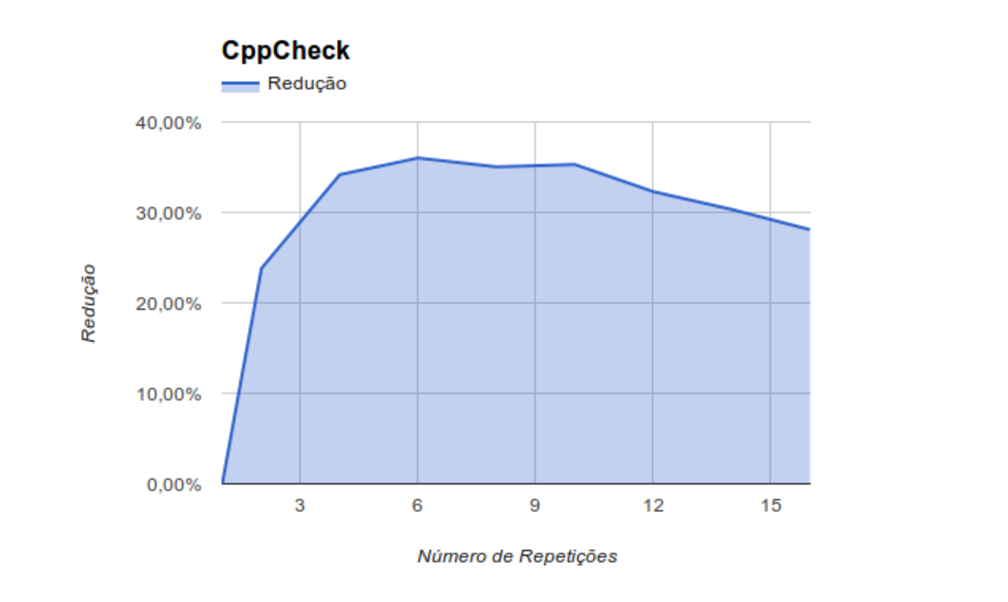
\includegraphics[keepaspectratio=true,scale=1]{figuras/cppcheck.eps}
    \caption{Redução do tempo de compilação para projeto CppCheck}
    \label{cppcheck}
\end{figure}
Analisando os resultados dos experimentos realizados com o projeto
 CppCheck, apresentados na tabela \ref{tab:cppcheck} e na Figura \ref{cppcheck},
 que indica um gráfico das porcentagens de redução, é
 possível afirmar que utilizar mais de uma thread para a
 compilação pode trazer uma redução no tempo de compilação.
 Neste projeto o beneficio da redução foi de 20\% a 35\%.
 É possível observar que o aumento das threads  não
 necessariamente aumenta a redução do tempo de compilação,
 uma vez que com 16 threads  a redução foi menor  do que com 12 threads.


\textbf{Hayai}


\begin{table}[h]
\centering
\caption{Hayai utilizando jobs do makefile}
\label{tab:hayai}
\begin{tiny}
\begin{tabular}{cccccccccc}
\toprule
\textbf{Repetições} & \multicolumn{9}{c}{\textbf{Número de threads}} \\ \midrule
- & 1 & 2 & 4 & 6 & 8 & 10 & 12 & 14 & 16 \\ 
1 & 3,443 & 2,964  & 2,523 &2,276 &2,624    & 2,612   &2,425    &2,389  &2,496  \\ 
2 & 3,287 & 2,43   & 2,374 &2,24  &2,53     & 2,66    &2,39     &2,748  &2,426   \\ 
3 & 3,622 & 2,531  & 2,489 &2,316 &2,673    & 2,737   &2,51     &2,46   &2,523 \\ 
4 & 3,456 & 2,906  & 2,468 &2,285 &2,534    & 2,399   &2,849    &2,707  &2,485 \\ 
5 & 3,816 & 2,498  & 2,466 &2,509 &2,568    & 2,416   &2,499    &2,718  &2,683 \\ 
6 & 3,757 & 2,415  & 2,457 &2,283 &2,735    & 2,539   &2,588    &2,584  &2,548 \\ 
7 & 3,504 & 2,604  & 2,549 &2,578 &2,621    & 2,621   &2,532    &2,398  &2,676 \\ 
8 & 3,404 & 2,451  & 2,433 &2,274 &2,533    & 2,683   &2,542    &2,502  &2,895 \\ 
9 & 3,564 & 2,474  & 2,886 &2,197 &2,902    & 2,399   &2,475    &2,82   &2,476 \\ 
10 & 3,482 & 2,571  & 2,458 &2,618 &2,618    & 2,623   &2,381    &2,755  &2,816 \\ \midrule
Média & 3,5335 &  2,5844 & 2,5103 & 2,357 & 2,6338 & 2,5689 & 2,5191 &2,6081 &2,6024 \\ \bottomrule
\end{tabular}
\end{tiny}
\end{table}

\begin{figure}[h]
    \centering
        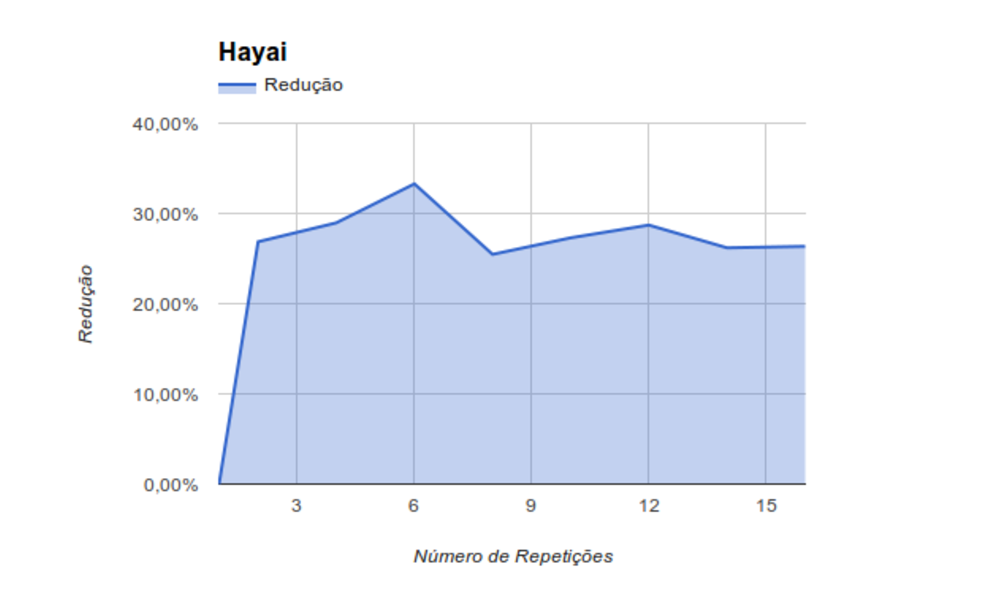
\includegraphics[keepaspectratio=true,scale=1]{figuras/hayai.eps}
    \caption{Redução do tempo de compilação para projeto Hayai}
    \label{hayai}
\end{figure}
Analisando os experimentos realizados com o hayai, utilizando a Tabela \ref{tab:hayai} e a Figura \ref{hayai} foi evidenciado ganho
 na redução do tempo de compilação do projeto, e com os mesmos
 observações do cppcheck. Neste caso com 16 threads foi maior que com
 12 threads. Neste projeto o ganho da redução do tempo de
 compilação varia entre 20\% e 32\%.

\textbf{JsonCpp}

\begin{table}[h]
\centering
\caption{JsonCpp utilizando jobs do makefile}
\label{tab:jsoncpp}
\begin{tiny}
\begin{tabular}{cccccccccc}
\toprule
\textbf{Repetições} & \multicolumn{9}{c}{\textbf{Número de threads}} \\ \midrule
- & 1 & 2 & 4 & 6 & 8 & 10 & 12 & 14 & 16 \\ 
1 & 16,013   & 11,599  & 11,117  & 9,838   & 12,202  & 10,114  & 11,366  & 10,966  & 12,108 \\
2 & 15,12    & 12,632  & 11,429  & 12,635  & 10,023  & 10,06   & 11,189  & 9,987   & 11,054 \\
3 & 14,932   & 11,967  & 10,48   & 10,098  & 11,136  & 11,24   & 9,862   & 10,177  & 10,285 \\
4 & 15,066   & 11,86   & 10,198  & 10,282  & 11,771  & 12,492  & 12,318  & 10,22   & 9,793 \\ 
5 & 15,202   & 11,383  & 10,112  & 10,882  & 10,714  & 10,476  & 9,991   & 10,917  & 10,033 \\
6 & 15,013   & 11,458  & 11,299  & 9,998   & 10,35   & 9,944   & 11,223  & 10,053  & 11,158 \\
7 & 14,98    & 11,519  & 10,909  & 9,95    & 11,481  & 11,105  & 11,071  & 11,19   & 11,288 \\
8 & 15,074   & 12,387  & 10,936  & 11,925  & 9,971   & 11,198  & 10,843  & 10,161  & 11,679 \\
9 & 15,361   & 11,668  & 11,74   & 11,229  & 12,218  & 10,222  & 10,551  & 10,019  & 9,879 \\ 
10 & 15,124   & 11,435  & 10,583  & 11,031  & 11,167  & 10,12   & 12,721  & 12,412  & 10,131 \\ \midrule
Média & 15,1885  & 11,7908 & 10,8803 & 10,7868 & 11,1033 & 10,6971 & 11,1135 & 10,6102 & 10,7408 \\ \bottomrule
\end{tabular}
\end{tiny}
\end{table}

\begin{figure}[h]
    \centering
        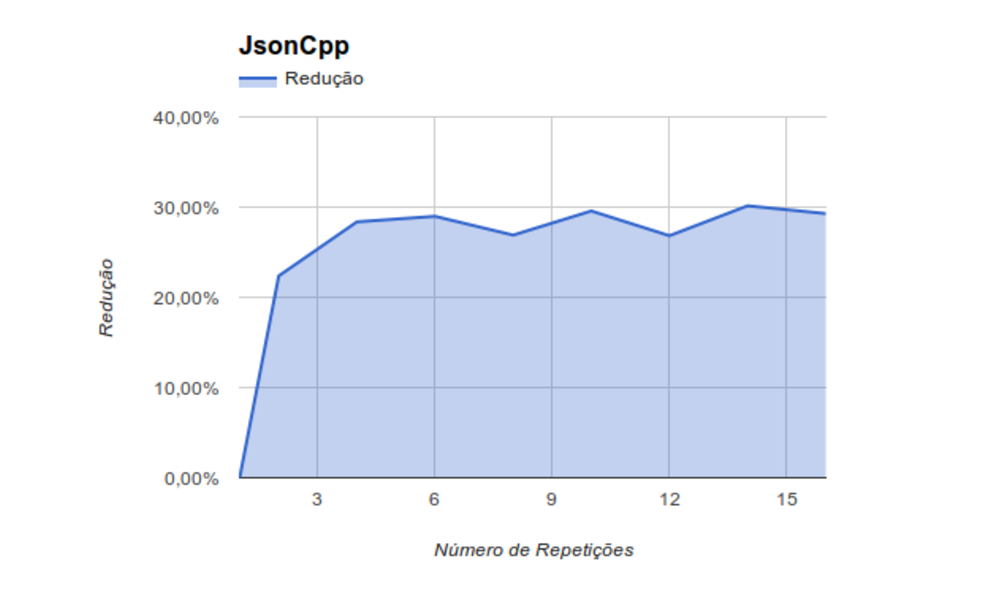
\includegraphics[keepaspectratio=true,scale=1]{figuras/jsoncpp.eps}
    \caption{Redução do tempo de compilação para projeto JsonCpp}
    \label{jsoncpp}
\end{figure}
Analisando os dados coletados no projeto Jsoncpp, como mostrado na Tabela \ref{tab:jsoncpp} e na Figura \ref{jsoncpp} é observado
 que o uso de thread proporciona
 redução do tempo de compilação, variando de 20\% a 31\%.
As mesmas observações encontradas no CppCheck.

\textbf{LibSass}

\begin{table}[h]
\centering
\caption{LibSass utilizando jobs do makefile}
\label{tab:libsass}
\begin{tiny}
\begin{tabular}{cccccccccc}
\toprule
\textbf{Repetições} & \multicolumn{9}{c}{\textbf{Número de threads}} \\ \midrule
- & 1 & 2 & 4 & 6 & 8 & 10 & 12 & 14 & 16 \\ 
1 & 52,448   & 42,562   & 32,535   & 42,828   & 31,111  & 31,391  & 31,625  & 31,508  & 31,965 \\ 
2 & 51,94    & 38,296   & 41,006   & 34,674   & 38,298  & 42,883  & 31,326  & 37,236  & 31,646 \\ 
3 & 51,632   & 39,621   & 43,227   & 33,82    & 31,341  & 47,873  & 32,94   & 32,237  & 39 \\ 
4 & 51,844   & 44,601   & 43,514   & 34,241   & 31,272  & 42,377  & 31,196  & 38,772  & 46,834 \\ 
5 & 51,165   & 38,335   & 33,511   & 43,01    & 38,582  & 47,222  & 31,56   & 46,99   & 34,354 \\ 
6 & 52,032   & 37,376   & 30,897   & 34,612   & 34,98   & 36,43   & 32,435  & 31,407  & 31,713 \\ 
7 & 51,525   & 36,105   & 42,818   & 30,831   & 36,641  & 37,691  & 40,757  & 38,838  & 31,59 \\ \
8 & 51,907   & 33,804   & 35,54    & 32,129   & 31,511  & 31,77   & 32,175  & 32,414  & 40,088 \\ 
9 & 51,79    & 43,258   & 31,919   & 30,811   & 34,529  & 47,326  & 32,586  & 39,355  & 38,228 \\ 
10& 52,046   & 40,352   & 46,493   & 37,484   & 42,191  & 41,195  & 31,749  & 37,03   & 31,607 \\ \midrule 
Média& 51,8329  & 39,431   & 38,146   & 35,444   & 35,0456 & 40,6158 & 32,8349 & 36,5787 & 35,7025 \\ \bottomrule
\end{tabular}
\end{tiny}
\end{table}

\begin{figure}[h]
    \centering
        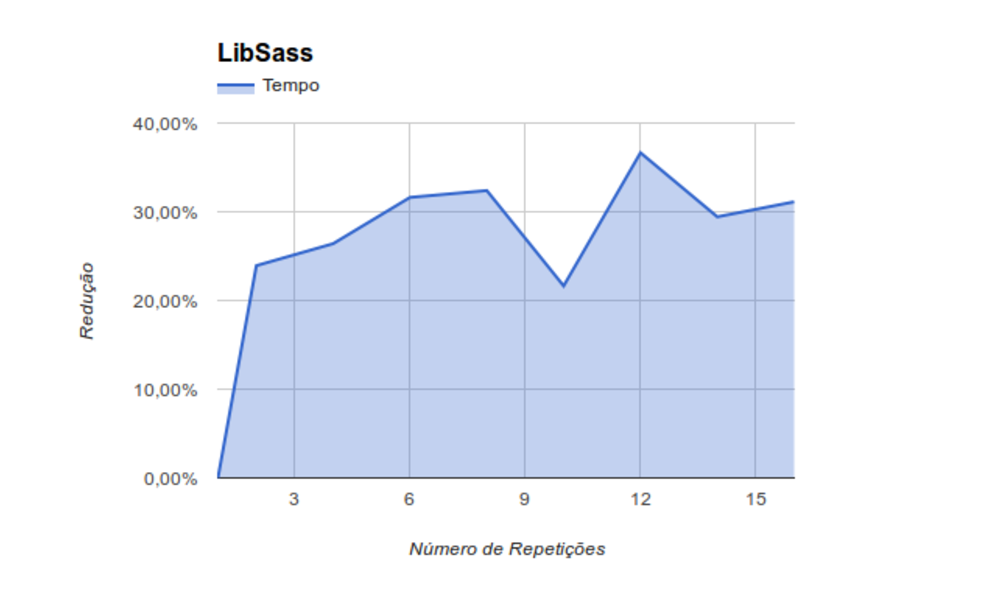
\includegraphics[keepaspectratio=true,scale=1]{figuras/libsass.eps}
    \caption{Redução do tempo de compilação para projeto LibSass}
    \label{libsass}
\end{figure}
Analisado as amostras para o projeto Libsass, como mostrado na Tabela \ref{tab:libsass} e na Figura \ref{libsass} é confirmado que o
 uso de threads reduziu o tempo de compilação e com variação
 de 20\% a 35\% de redução do tempo de compilação.

\textbf{LibOAuthCpp}

\begin{table}[h]
\centering
\caption{LibOAuthCpp utilizando jobs do makefile}
\label{tab:liboauthcpp}
\begin{tiny}
\begin{tabular}{cccccccccc}
\toprule
\textbf{Repetições} & \multicolumn{9}{c}{\textbf{Número de threads}} \\ \midrule
- & 1 & 2 & 4 & 6 & 8 & 10 & 12 & 14 & 16 \\ 
1 & 13,057   & 12,295   & 12,289   & 12,217   &  11,632   &  11,743  &  12,406  &   12,116  &   11,798 \\ 
2 & 13,213   & 12,218   & 12,368   & 11,682   &  12,181   &  11,792  &  11,716  &   12,224  &   11,681 \\ 
3 & 13,302   & 11,689   & 12,149   & 12,007   &  12,038   &  11,724  &  11,993  &   12,458  &   11,821 \\ 
4 & 13,054   & 12,219   & 11,987   & 12,071   &  11,614   &  11,722  &  11,702  &   11,662  &   12,069 \\ 
5 & 13,113   & 12,261   & 12,073   & 11,671   &  12,345   &  11,988  &  11,662  &   11,935  &   11,651 \\ 
6 & 13,392   & 12,109   & 11,908   & 11,753   &  12,402   &  11,812  &  12,366  &   11,732  &   12,066 \\ 
7 & 13,125   & 12,012   & 12,075   & 11,809   &  11,614   &  11,707  &  12,304  &   12,333  &   11,679 \\ 
8 & 13,241   & 11,981   & 11,725   & 11,762   &  11,847   &  12,426  &  12,043  &   12,588  &   11,993 \\ 
9 & 13,021   & 12,09    & 11,864   & 11,708   &  11,904   &  12,014  &  12,709  &   12,151  &   12,007 \\ 
10 & 13,644   & 12,348   & 12,267   & 12,288   &  12,251   &  11,884  &  12,56   &   11,892  &   12,557 \\ \midrule
Média & 13,2162  & 12,1222  & 12,0705  & 11,8968  &  11,9828  &  11,8812 &  12,1461 &   12,1091 &   11,9322 \\ \bottomrule
\end{tabular}
\end{tiny}
\end{table}

\begin{figure}[h]
    \centering
        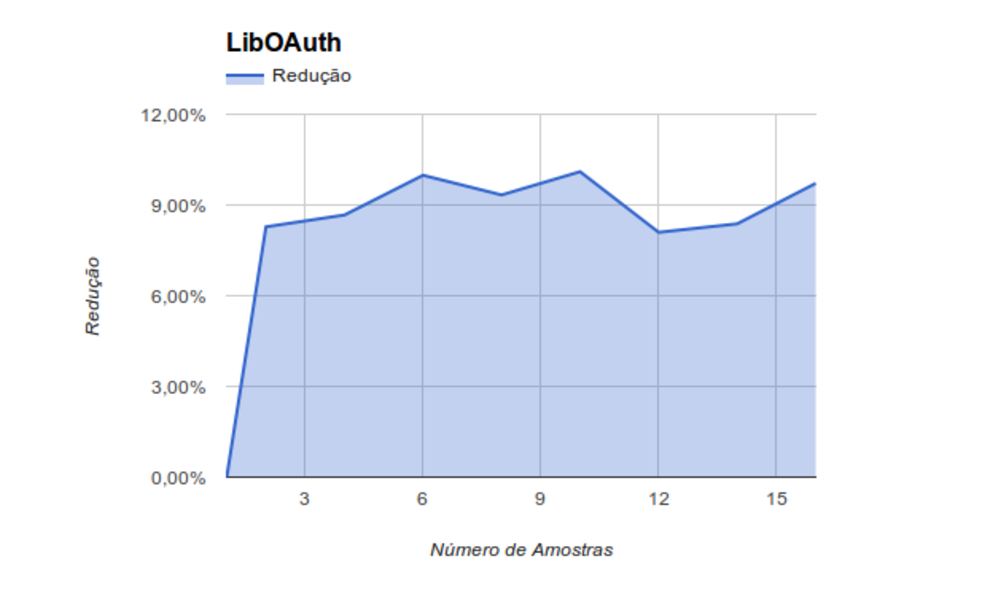
\includegraphics[keepaspectratio=true,scale=1]{figuras/liboauth.eps}
    \caption{Redução do tempo de compilação para projeto LibOAuth}
    \label{liboauthcpp}
\end{figure}
Analisando a coleta de dados do projeto LibOAuth, como mostrado na Tabela \ref{tab:liboauthcpp} e na Figura \ref{liboauthcpp} é evidenciado que ele possui
 redução do tempo de compilação , no entanto este projeto não teve ganhos
 acima de 10\%. Este valores são totalmente diferentes dos outros projetos,
 então a estrutura do projeto pode ter influenciado na redução do
 tempo de compilação. 

\textbf{Jack, the Janitor}

\begin{table}[h]
\centering
\caption{Jack, the Janitor utilizando jobs do makefile}
\label{tab:jack}
\begin{tiny}
\begin{tabular}{cccccccccc}
\toprule
\textbf{Repetições} & \multicolumn{9}{c}{\textbf{Número de threads}} \\ \midrule
- & 1 & 2 & 4 & 6 & 8 & 10 & 12 & 14 & 16 \\ 
1 & 5,21    & 2,24  &  2,13   & 2,15   & 2,19   & 2,32   & 2,41  &  2,73  & 2,25 \\ \hline
2 & 3,92    & 2,44  &  2,73   & 2,21   & 2,24   & 2,23   & 2,38  &  2,33  & 2,29 \\ \hline
3 & 3,94    & 2,51  &  2,84   & 2,28   & 2,24   & 2,27   & 2,22  &  2,34  & 3,01 \\ \hline
4 & 4,02    & 2,64  &  2,46   & 2,22   & 2,22   & 2,19   & 2,28  &  2,23  & 2,26 \\ \hline
5 & 3,87    & 2,51  &  2,32   & 2,29   & 2,64   & 2,51   & 2,25  &  2,33  & 2,74 \\ \hline
6 & 3,81    & 2,91  &  2,30   & 2,27   & 2,63   & 2,30   & 2,26  &  2,23  & 3,14 \\ \hline
7 & 3,91    & 2,40  &  2,28   & 2,17   & 2,40   & 3,09   & 2,74  &  2,33  & 2,35 \\ \hline
8 & 3,88    & 2,39  &  2,52   & 2,34   & 2,34   & 2,31   & 2,27  &  2,31  & 3,00 \\ \hline
9 & 3,93    & 2,54  &  2,87   & 2,38   & 2,31   & 2,26   & 3,02  &  2,37  & 2,40 \\ \hline
10 & 3,84    & 3,10  &  2,85   & 2,23   & 2,22   & 2,18   & 2,75  &  2,35  & 3,04 \\ \hline
Média & 4,0308  & 2,5651&  2,5293 & 2,2547 & 2,3426 & 2,3657 & 2,4565&  2,3529 & 2,6473 \\ \hline
\end{tabular}
\end{tiny}
\end{table}
\begin{figure}[h]
    \centering
        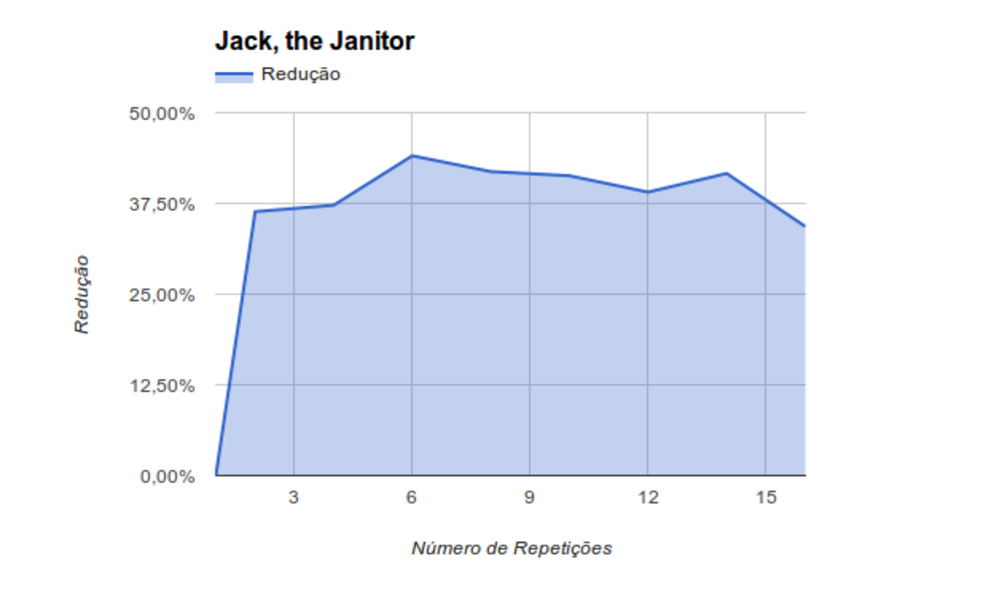
\includegraphics[keepaspectratio=true,scale=1]{figuras/jack.eps}
    \caption{Redução do tempo de compilação para projeto Jack, the Janitor}
    \label{jack}
\end{figure}
Analisando os dados coletados do projeto Jack, the Janitor,
 como mostrado na Tabela \ref{tab:jack} e na Figura \ref{jack}
 percebemos as mesmas reduções entre os projetos anteriores
 e ainda mais neste projeto as os ganhos da redução do
 tempo de compilação foram maiores.

Após a coleta dos dados dos 6 projetos distintos podemos
 perceber que não há uma relação direta entre as diferentes
 quantidades de threads. Isto é observado nos gráficos,
 com o aumento das threads não necessariamente implicando
 em um aumento proporcional. Os dados encontrados
 sugerem que este método pode reduzir o tempo de
 compilação em aproximadamente 20\%.
